\let\negmedspace\undefined
\let\negthickspace\undefined
\documentclass[journal]{IEEEtran}
\usepackage[a5paper, margin=10mm, onecolumn]{geometry}
%\usepackage{lmodern} % Ensure lmodern is loaded for pdflatex
\usepackage{tfrupee} % Include tfrupee package

\setlength{\headheight}{1cm} % Set the height of the header box
\setlength{\headsep}{0mm}     % Set the distance between the header box and the top of the text

\usepackage{gvv-book}
\usepackage{gvv}
\usepackage{cite}
\usepackage{amsmath,amssymb,amsfonts,amsthm}
\usepackage{algorithmic}
\usepackage{graphicx}
\usepackage{textcomp}
\usepackage{xcolor}
\usepackage{txfonts}
\usepackage{listings}
\usepackage{enumitem}
\usepackage{mathtools}
\usepackage{gensymb}
\usepackage{comment}
\usepackage[breaklinks=true]{hyperref}
\usepackage{tkz-euclide} 
\usepackage{listings}
% \usepackage{gvv}                                        
\def\inputGnumericTable{}                                 
\usepackage[latin1]{inputenc}                                
\usepackage{color}                                            
\usepackage{array}                                            
\usepackage{longtable}                                       
\usepackage{calc}                                             
\usepackage{multirow}                                         
\usepackage{hhline}                                           
\usepackage{ifthen}                                           
\usepackage{lscape}
\begin{document}

\bibliographystyle{IEEEtran}
\vspace{3cm}

\title{1-1.8-21}
\author{EE24BTECH11060 - Sruthi Bijili}
% \maketitle
% \newpage
% \bigskip
{\let\newpage\relax\maketitle}

\renewcommand{\thefigure}{\theenumi}
\renewcommand{\thetable}{\theenumi}
\setlength{\intextsep}{10pt} % Space between text and floats


\numberwithin{equation}{enumi}
\numberwithin{figure}{enumi}
\renewcommand{\thetable}{\theenumi}

\textbf{Question}:\\
Find a point which is equidistant from the points \brak{-5, 4} and \brak{-1,6}. How many such points are there ?

\textbf{solution}:\\
\begin{table}[h!]    
  \centering
  \begin{tabular}[12pt]{ |c| c|}
    \hline
        \textbf{Variable}  & \textbf{Description} \\
    \hline
        $\vec{A}$$\brak{-5,4}$ &  coordinates of first point \\
    \hline 
        $\vec{B}$$\brak{-1,6}$ & coordinates of second point \\
    \hline
        $\vec{C}$& midpoint of $\vec{A}$ and $\vec{B}$ \\ 
    \hline       
\end{tabular}

  \caption{Variables Used}
  \label{tab1.1.8.21}
\end{table}
\begin{align}
\abs{\abs{\vec{C}-\vec{A}}}&=\abs{\abs{\vec{C}-\vec{B}}}\\
\implies\abs{\abs{\vec{C}-\vec{A}}}^2&=\abs{\abs{\vec{C}-\vec{B}}}^2\\
\implies\abs{\abs{\vec{C}}}^2-2\vec{C}^T\vec{A}+\abs{\abs{\vec{A}}}^2&=\abs{\abs{\vec{C}}}^2-2\vec{C}^T\vec{B}+\abs{\abs{\vec{B}}}^2\\
\implies\brak{A-B}^2\vec{C}&=\frac{\abs{\abs{\vec{A}}}^2-\abs{\abs{\vec{B}}}^2}{2}\\
\text{ by substituting the values from table}\\
\implies 2x+y&=-1\\
\text{if} x&=-3\\
\implies y&=5\\
\vec{C}&=\myvec{-3 \\ 5}
\end{align}
\text{There are infinitely many points that are equidistant from the points\brak{-5,4} and \brak{-1,6}}
\begin{figure}[h!]
   \centering
   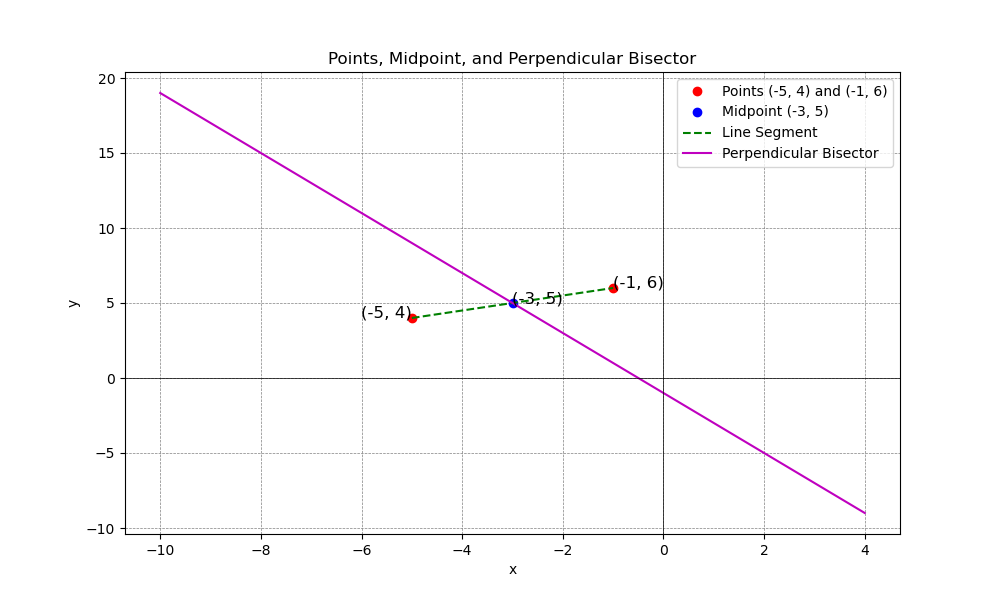
\includegraphics[width=0.7\linewidth]{figs/fig1.png}
   \caption{line passing through the midpoint of AB}
\end{figure}

\end{document}
